% Copyright 2026 Sreeram Anil
% SPDX-License-Identifier: CC-BY-4.0
% =============================================================================
%  U-D factorised Kalman filter (Bierman-Thornton) — classical Kalman family
% =============================================================================
\chapter{U-D Factorised Kalman Filter (UD-EKF)}
\label{ch:udekf}

\section*{At a glance}
\begin{tabular}{@{}l>{\raggedright\arraybackslash}p{0.76\textwidth}@{}}
Family & classical Kalman (factored) \\
Header & \texttt{include/estkit/filters/udkf.hpp} \\
Registered name & \texttt{UD-EKF} \\
State dimension & $n_x = 4$ (cell model) --- generic in $n_x, n_u, n_y$ \\
Propagated quantities & $\mU$ unit upper triangular, $\mD$ diagonal, $\mP = \mU\mD\mU^\T$ \\
Cost per step & $\mathcal{O}(n_x^2(n_x{+}n_q))$, no square roots; $0.45$--$0.49\,\SI{}{\micro\second}$/step \\
Primary references & \cite{bierman1977,thornton1976ud,kaminski1971,grewal2014,verhaegen1986} \\
\end{tabular}

\section{Motivation and aerospace/BMS relevance}
The U-D filter is the square-root filter without the square roots. Bierman observed that the
numerical benefit of factoring $\mP$ comes from working with a factor whose condition number
is $\sqrt{\kappa(\mP)}$, and that a Cholesky factor is not the only such object: the
factorisation $\mP = \mU\mD\mU^\T$, with $\mU$ unit upper triangular and $\mD$ diagonal and
non-negative, has the same conditioning and needs only multiplies and divides. On the
fixed-point and early floating-point machines of the 1970s that was decisive, and the
Bierman--Thornton pair (scalar measurement update~\cite[Ch.~V]{bierman1977}, modified weighted
Gram--Schmidt time update~\cite{thornton1976ud}) became the standard formulation for JPL deep
space navigation, for GPS receivers, and for the Space Shuttle navigation filter. It is still
the reference implementation in Grewal and Andrews~\cite{grewal2014} and remains the
formulation most often found in certified embedded navigation software.

For a BMS the argument is the same as for the square-root EKF, with one addition: many
automotive and aerospace battery controllers still use fixed-point DSP cores or software
floating point, where a square root costs tens of cycles. The U-D filter has exactly one
division per state per scalar measurement and no transcendental operations at all.

\section{Problem statement and assumptions}
Model \eqref{eq:ekf-proc}--\eqref{eq:ekf-meas}. The filter maintains
\begin{equation}
\mP = \mU\mD\mU^\T, \qquad
\mU = \begin{bmatrix}1 & u_{12} & \cdots\\ 0 & 1 & \\ & & \ddots\end{bmatrix},\quad
\mD = \diag(d_1,\dots,d_{n_x}),\; d_i\ge0 .
\label{eq:ud-def}
\end{equation}
The measurement update processes one scalar component at a time. For that to be exact rather
than approximate, the measurement noise of the components must be independent; when $\mR$ is
not diagonal the components are first decorrelated (below). No positive-definiteness
assumption is needed beyond $\mD\succeq0$, which the algorithm preserves by construction.

\section{Derivation}
\paragraph{U-D factorisation.} For a symmetric positive semi-definite $\bm{M}$, comparing
entries of $\bm{M} = \mU\mD\mU^\T$ from the bottom-right corner upwards gives the recursion
\begin{equation}
d_j = m_{jj} - \sum_{k>j} u_{jk}^2 d_k, \qquad
u_{ij} = \frac{1}{d_j}\left(m_{ij} - \sum_{k>j} u_{ik}\,d_k\,u_{jk}\right), \quad i<j,
\label{eq:ud-factor}
\end{equation}
processed for $j = n_x, n_x-1,\dots,1$~\cite[App.~III]{bierman1977}. It costs
$\mathcal{O}(n_x^3/6)$ and no square roots.

\paragraph{Bierman's scalar measurement update.} Let the scalar observation be
$y = \bm a^\T\vx + v$, $\Var{v} = r$. Substituting $\mP = \mU\mD\mU^\T$ into the Kalman update
and requiring the result to be in U-D form again yields a recursion in which the innovation
variance is built up one state at a time. With
\begin{equation}
\bm f = \mU^\T\bm a \;(\text{so } f_j = \sum_{i\le j} u_{ij}a_i), \qquad
\bm b = \mD\bm f \;(\text{so } b_j = d_j f_j),
\label{eq:ud-fb}
\end{equation}
set $\alpha_0 = r$ and, for $j = 1,\dots,n_x$,
\begin{align}
\alpha_j &= \alpha_{j-1} + f_j b_j, &
d_j &\leftarrow d_j\,\frac{\alpha_{j-1}}{\alpha_j}, &
\lambda_j &= -\frac{f_j}{\alpha_{j-1}},
\label{eq:ud-bierman1}\\
u_{ij} &\leftarrow u_{ij} + \lambda_j b_i, &
b_i &\leftarrow b_i + u_{ij}^{\text{old}}\,b_j, & &\quad i<j .
\label{eq:ud-bierman2}
\end{align}
After the sweep, two identities hold and are the reason the algorithm works:
\begin{equation}
\alpha_{n_x} = \bm a^\T\mP\bm a + r = \mS \quad\text{(innovation variance)},\qquad
\bm b = \mP\bm a \quad\text{(unnormalised gain)},
\label{eq:ud-identities}
\end{equation}
so the state update is $\xhat \leftarrow \xhat + (\bm b/\alpha_{n_x})(y - \bm a^\T\xhat)$. The
updated $\mU,\mD$ are produced in place. Every $\alpha_j$ is a sum of non-negative terms
($f_jb_j = d_jf_j^2 \ge 0$) added to $r>0$, so no cancellation can make it non-positive: the
update cannot produce a negative variance. The cost is $\mathcal{O}(n_x^2)$ per scalar
measurement with exactly $n_x$ divisions.

\paragraph{Decorrelation for vector measurements.} If $\mR$ is not diagonal, factor
$\mR = \mL_R\mL_R^\T$ and replace $(\mH,\bm\veps)$ by
$(\mL_R\inv\mH,\ \mL_R\inv\bm\veps)$; the transformed components have unit, independent
variances and \eqref{eq:ud-bierman1}--\eqref{eq:ud-bierman2} applies to each in turn with
$r=1$~\cite[\S V.4]{bierman1977}. When components are processed sequentially the state moves
between them, so the $k$-th residual must be taken at the \emph{current} state,
$\delta z_k = \tilde\veps_k - \tilde{\bm a}_k^\T(\xhat - \xminus)$, which for a linearised
model makes sequential processing exactly equivalent to a simultaneous vector update.

\paragraph{Thornton's modified weighted Gram--Schmidt time update.} Write
$\mQ = \mG\mD_q\mG^\T$ (itself a U-D factorisation, so a fully correlated $\mQ$ is admissible)
and stack
\begin{equation}
\mW = \left[\ \mF\mU \;\;\; \mG\ \right] \in \real^{n_x\times(n_x+n_q)}, \qquad
\mD_w = \diag\!\left(\mD,\ \mD_q\right),
\label{eq:ud-thornton-setup}
\end{equation}
so that $\Pminus = \mW\mD_w\mW^\T$. Applying \emph{weighted} Gram--Schmidt to the ROWS of
$\mW$, orthogonalising from the last row upwards, gives
\begin{equation}
d^-_i = \sum_k W_{ik}^2 (\mD_w)_k, \qquad
u^-_{ji} = \frac{1}{d^-_i}\sum_k W_{ik}(\mD_w)_k W_{jk}, \qquad
W_{j:} \leftarrow W_{j:} - u^-_{ji}W_{i:}, \quad j<i,
\label{eq:ud-thornton}
\end{equation}
for $i = n_x,\dots,1$. Because row $i$ is finalised before it is used to reduce rows $j<i$,
the original array satisfies $\mW_{\text{orig}} = \mU^-\mW_{\text{final}}$ with
$\mU^-$ unit upper triangular, and the rows of $\mW_{\text{final}}$ are $\mD_w$-orthogonal
with $\mD_w$-norms $d^-_i$; hence
$\Pminus = \mW_{\text{orig}}\mD_w\mW_{\text{orig}}^\T = \mU^-\mD^-\mU^{-\T}$ as
required~\cite{thornton1976ud}. Cost: $\mathcal{O}(n_x^2(n_x+n_q))$, again with no square
roots.

\section{Algorithm}
\begin{algorithm}[H]
\caption{UD-EKF (Bierman--Thornton) --- one sampling period}
\begin{algorithmic}[1]
\Require $\xplus_{k-1},\mU^+_{k-1},\mD^+_{k-1},\vu_{k-1},\vy_k,\vu_k$
\State \textbf{Time update (Thornton):} $\mF\gets\partial f/\partial\vx|_{\xplus_{k-1},\vu_{k-1}}$;\;
       $\xminus_k\gets f(\xplus_{k-1},\vu_{k-1})$
\State $(\mG,\mD_q)\gets\text{UD}(\mQ)$;\;
       $\mW\gets[\mF\mU^+_{k-1}\;\;\mG]$;\; $\mD_w\gets\diag(\mD^+_{k-1},\mD_q)$
\For{$i=n_x$ \textbf{down to} $1$}
  \State $d^-_i\gets\sum_k W_{ik}^2(\mD_w)_k$
  \For{$j=1,\dots,i-1$}
    \State $u^-_{ji}\gets\left(\sum_k W_{ik}(\mD_w)_kW_{jk}\right)/d^-_i$;\;
           $W_{j:}\gets W_{j:}-u^-_{ji}W_{i:}$
  \EndFor
\EndFor
\State \textbf{Predicted measurement:} $\yhat_k\gets h(\xminus_k,\vu_k)$
\State \textbf{Measurement update (Bierman):} $\mH\gets\partial h/\partial\vx|_{\xminus_k,\vu_k}$;\;
       decorrelate if $\mR$ is not diagonal
\For{$k'=1,\dots,n_y$}
  \State $\bm a\gets$ row $k'$ of $\mH$;\; $\delta z\gets\tilde\veps_{k'}-\bm a^\T(\xhat-\xminus_k)$
  \State apply \eqref{eq:ud-fb}--\eqref{eq:ud-bierman2};\;
         $\xhat\gets\xhat+(\bm b/\alpha_{n_x})\,\delta z$
\EndFor
\State \textbf{if} constraints enabled \textbf{then} $\xplus_k\gets\Pi(\xhat)$
\Ensure $\xplus_k,\mU^+_k,\mD^+_k$ \quad ($\mP$ reconstructed on demand as $\mU\mD\mU^\T$)
\end{algorithmic}
\end{algorithm}

\section{Application to the battery model}
$n_y=1$, so the Bierman sweep runs once per sample: four multiplies for $\bm f = \mU^\T\bm a$,
four for $\bm b$, then four iterations of \eqref{eq:ud-bierman1}--\eqref{eq:ud-bierman2} ---
about $40$ multiply-accumulates and $4$ divisions in total. $\mF$ is diagonal, so
$\mF\mU$ is a row scaling. $\mQ$ is \emph{not} diagonal (it carries the rank-one
current-noise term $\bm b\bm b^\T\sigma_i^2$), which is exactly the case Thornton's algorithm
was designed for: the U-D factorisation of $\mQ$ supplies $\mG$ and $\mD_q$ and the
Gram--Schmidt pass handles the correlation without any special casing. The work array $\mW$ is
$4\times8$.

Options: \code{decorrelate = true} (inactive at $n_y=1$), \code{apply\_constraints = true},
\code{q\_scale = r\_scale = 1}, \code{d\_floor = 0} (a lower bound that can be raised to keep
the filter from becoming arbitrarily confident in a state).

\section{Implementation notes}
The U-D filter is the fastest of the EKF-equivalent implementations, at
$0.45$--$0.49\,\SI{}{\micro\second}$ per step against the square-root EKF's $0.78$--$0.83$ and
the information filter's $1.17$--$1.24$, and indistinguishable from the conventional EKF's
$0.44$--$0.48$: it replaces two Householder QRs by one Gram--Schmidt pass and one scalar sweep
and uses no square roots at all. Only the frozen-linearisation LKF ($320$--$336$\,ns) is
faster, and it is a different estimator. That the factored form costs nothing relative to the
conventional one is the historical selling point of the formulation, and it survives unchanged
on modern hardware.

Numerical guards: $d_j$ is clamped to $\ge$ \code{d\_floor} after each update; an
$\alpha_j$ that fails to be positive (possible only through a corrupted $d_j$) leaves the
state untouched for that index; the gain application is skipped if $\delta z/\alpha$ is not
finite. The U-D factorisation \eqref{eq:ud-factor} sets $d_j = 0$ and $u_{ij} = 0$ rather than
dividing by a non-positive pivot. $\mP$ is exposed through a cached $\mU\mD\mU^\T$ product for
the benchmark's $\sigma_\soc$ reporting; a flight implementation would read
$\sigma_\soc^2 = \sum_j u_{1j}^2 d_j$ directly.
\code{sizeof(UdKf<EcmModel>)} is 4480\,bytes.

Verification: the U-D factorisation was checked against a dense reconstruction
($\max\abs{\mU\mD\mU^\T-\bm{M}} = 2.2\times10^{-16}$ on a $4\times4$ test matrix), and the
complete filter against the EKF over a full mission.

\section{Benchmark results}
\input{tables/cell_UDEKF.tex}
\begin{figure}[H]\centering
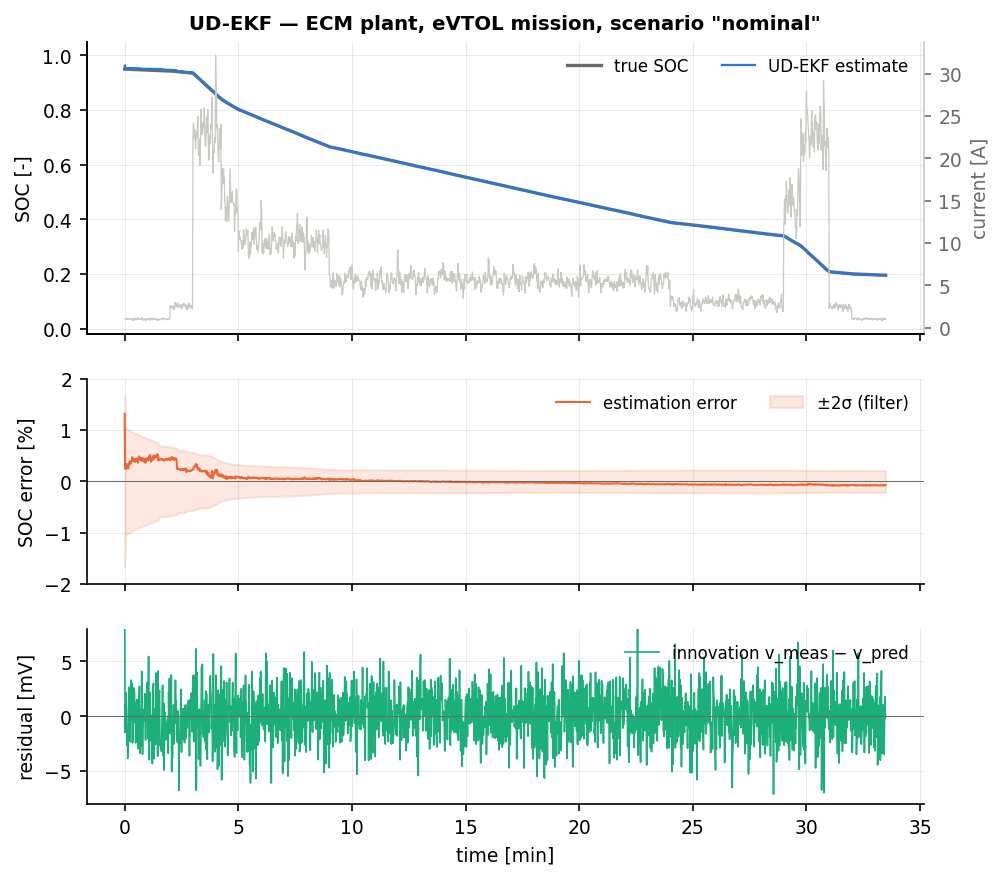
\includegraphics[width=\textwidth]{figures/cell_UDEKF_nominal.png}
\caption{UD-EKF on the nominal eVTOL mission: true and estimated SOC (top), estimation error with the $\pm 2\sigma$ band when available (middle), voltage residual (bottom).}
\end{figure}
\begin{figure}[H]\centering
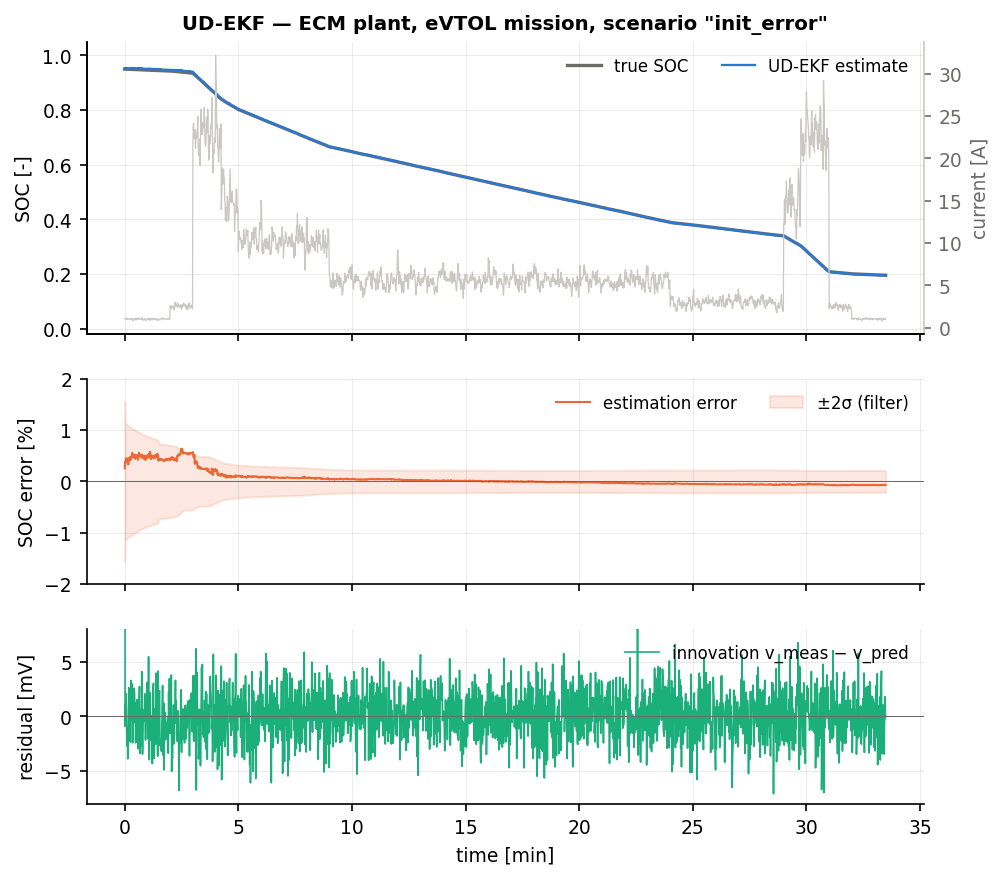
\includegraphics[width=\textwidth]{figures/cell_UDEKF_init_error.png}
\caption{UD-EKF with a 35\,\% initial SOC error.}
\end{figure}

All numbers are three-seed means in per cent SOC.

The UD-EKF reproduces the EKF on all twelve ECM scenarios to two decimals --- \texttt{nominal}
$0.15/0.05\,\%$, \texttt{init\_error} $0.14/0.05\,\%$ with $t_{\text{conv}} = 0$\,s,
\texttt{current\_bias} $0.54/0.61\,\%$, \texttt{outliers} $0.52/0.21\,\%$, \texttt{aged\_cell}
$1.18/1.52\,\%$, \texttt{param\_mismatch} $1.28/1.36\,\%$, \texttt{sensor\_dropout}
$0.72/0.46\,\%$, \texttt{preisach} $0.58/0.20\,\%$, \texttt{combined} $16.02/12.44\,\%$ (never
converges) --- with an element-wise agreement of $\max\abs{\Delta\vx} = 1.6\times10^{-14}$ and
$\max\abs{\Delta\mP} = 7.6\times10^{-16}$ over $\num{18000}$ steps. The covariance agreement is
the tightest of the three EKF-equivalent implementations in this family (SR-EKF
$4.0\times10^{-15}$, EIF $1.3\times10^{-14}$), which is consistent with the U-D form never
forming $\mP$ and never taking a square root. The estimation discussion of
Chapter~\ref{ch:ekf} applies unchanged.

What distinguishes this chapter from the SR-EKF's is the cost column. The U-D filter is
\emph{free} relative to the conventional covariance form --- $0.45$--$0.49\,\SI{}{\micro\second}$
against the EKF's $0.44$--$0.48$, a difference of a few nanoseconds and well inside the
run-to-run spread --- while providing the guarantee that $\mP$ cannot go indefinite
($\mD\succeq0$ is enforced elementwise). The square-root EKF costs $70\,\%$ more for the same
guarantee. There is, on this evidence, no reason to prefer the conventional covariance EKF over
the U-D form in an embedded implementation: it costs the same, is better conditioned, needs no
square roots, and produces the same numbers. In single precision the two are also
indistinguishable ($0.06\,\%$ on \texttt{nominal}, $1.48\,\%$ on \texttt{aged\_cell},
$12.18\,\%$ on \texttt{combined} against the EKF's $12.21\,\%$).

Two caveats. First, the advantage is specific to $n_y\ll n_x$: the Bierman sweep costs
$\mathcal{O}(n_x^2)$ per scalar measurement, so with many simultaneous measurements the
$\mathcal{O}(n_yn_x^2)$ total overtakes a single batched update; the square-root array form of
Chapter~\ref{ch:srekf} handles a vector measurement in one pass and is preferable there.
Second, in the artificial ill-conditioning stress test described in Chapter~\ref{ch:srekf}
(float build, $\mR$ scaled by $10^{-4}$) the U-D filter came out at
$\text{RMSE}_{\text{ss}} = 5.07\,\%$ against the SR-EKF's $0.79\,\%$ and the EKF's $2.39\,\%$;
since all three are algebraically identical this reflects the chaotic sensitivity of that
deliberately broken configuration rather than a conditioning ranking, and no conclusion should
be drawn from it beyond ``do not trust a filter whose $\mR$ is wrong by four orders of
magnitude''.

\paragraph{SPM plant: structured model error.}
\begin{figure}[H]\centering
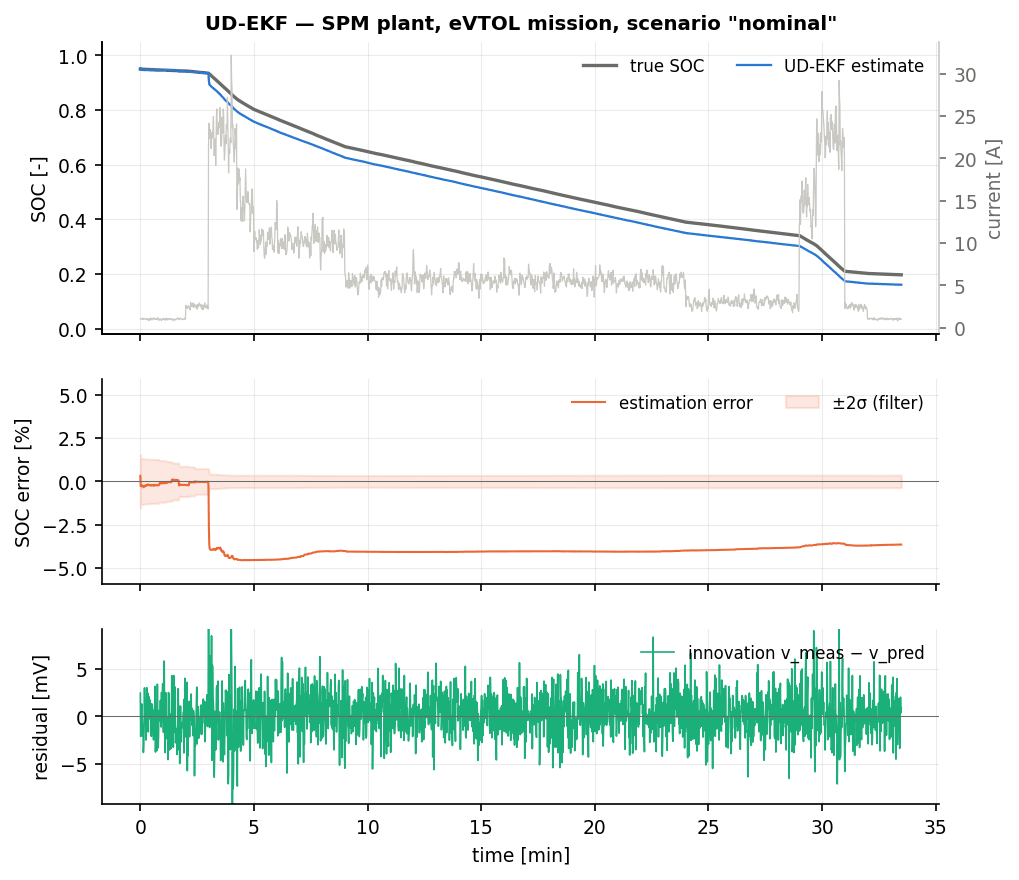
\includegraphics[width=\textwidth]{figures/cellspm_UDEKF_nominal.png}
\caption{UD-EKF on the nominal mission with the electrochemical (SPM) plant; identical to the conventional EKF.}
\end{figure}
The SPM block of the table is a different kind of test. The plant is the electrochemical
single-particle model; the estimator still runs a 2-RC equivalent circuit, fitted to that plant,
which leaves a \emph{structured} residual of about $4$\,mV (Butler--Volmer kinetics and
solid-phase diffusion that no 2-RC circuit can reproduce) and a slow second branch,
$\tau_2 = 556$\,s. Over a $33$-minute mission a $556$\,s pole barely relaxes, so $v_2(t)$ is
close to an affine ramp --- and so is $\ocv(\soc(t))$ while the cell discharges at a roughly
constant rate. The two channels through which the measurement sees the state,
$(\partial\ocv/\partial\soc)\,\delta\soc$ and $-\delta v_2$, are therefore nearly collinear in
the information accumulated over the flight: the pair $(\soc, v_2)$ is close to unobservable,
and no filter can decide whether a persistent few-millivolt residual belongs to the slow RC
branch or to the state of charge. Because that direction is weakly observable, a $4$\,mV
structured error maps onto \emph{several per cent} of SOC instead of the
$4\,\text{mV}/0.8\,\text{V}\approx0.5\,\%$ a well-conditioned channel would give. This
$(\soc,v_2)$ ambiguity, not the size of the residual, is the mechanism behind the
$3.7$--$4.6\,\%$ band in which the whole classical family sits.

Being algebraically the EKF, this filter inherits the EKF's SPM rows exactly:
$3.65/3.73\,\%$ on \texttt{nominal} with a voltage residual of only $1.02$\,mV,
$7.35\,\%$ on \texttt{cold}, $5.69\,\%$ on \texttt{current\_bias}, $5.31\,\%$ on
\texttt{sensor\_dropout}, $3.13\,\%$ on \texttt{param\_mismatch} and $1.99\,\%$ on
\texttt{outliers}. Fitting the voltage to a millivolt while being $4\,\%$ wrong about SOC is
the signature of the ambiguity: the filter pays for the fit with $v_2$ and $\soc$ in the wrong
proportion. Nothing diverges and $t_{\text{conv}} = 0$ on every SPM row --- the error is a
bias, not a drift. Within the family the tangent-linearising filters (EKF, IEKF and these three
re-implementations) are at the \emph{good} end of the band, because a tangent commits less
weight to the badly conditioned OCV channel than a wide statistical regression does; only the
frozen-linearisation LKF ($1.72\,\%$, Chapter~\ref{ch:lkf}) and the second-order EKF
($3.52\,\%$) do better.

\section{Summary}
The Bierman--Thornton U-D filter is the implementation of choice for an embedded EKF: it gives
bit-for-bit the EKF's estimates, guarantees a non-negative covariance by construction, uses no
square roots and no matrix inversions, and on this benchmark costs exactly what the conventional
EKF costs. Use it for any fixed-point or software-floating-point target, for any application
where a negative variance must be impossible by construction, and by default whenever
$n_y\ll n_x$. Its limitation is the scalar measurement sweep, which becomes the bottleneck when
many measurements arrive simultaneously; and, being an EKF, it inherits the EKF's
over-confidence on curved measurement functions (\texttt{combined}) and the EKF's $4\,\%$ bias
under structured model error (the SPM rows).
